%%%%%%%%%%%%%%%%%%%%%%%%%%%%%%%%%%%%%%%%%
% a0poster Portrait Poster
% LaTeX Template
% Version 1.0 (22/06/13)
%
% The a0poster class was created by:
% Gerlinde Kettl and Matthias Weiser (tex@kettl.de)
% 
% This template has been downloaded from:
% http://www.LaTeXTemplates.com
%
% License:
% CC BY-NC-SA 3.0 (http://creativecommons.org/licenses/by-nc-sa/3.0/)
%
%%%%%%%%%%%%%%%%%%%%%%%%%%%%%%%%%%%%%%%%%

%----------------------------------------------------------------------------------------
%	PACKAGES AND OTHER DOCUMENT CONFIGURATIONS
%----------------------------------------------------------------------------------------

\documentclass[a0,portrait]{a0poster}

\usepackage{multicol} % This is so we can have multiple columns of text side-by-side
\columnsep=100pt % This is the amount of white space between the columns in the poster
\columnseprule=3pt % This is the thickness of the black line between the columns in the poster

\usepackage[svgnames]{xcolor} % Specify colors by their 'svgnames', for a full list of all colors available see here: http://www.latextemplates.com/svgnames-colors

\usepackage{times} % Use the times font
%\usepackage{palatino} % Uncomment to use the Palatino font

\usepackage{graphicx} % Required for including images
\graphicspath{{figures/}} % Location of the graphics files
\usepackage{booktabs} % Top and bottom rules for table
\usepackage[font=small,labelfont=bf]{caption} % Required for specifying captions to tables and figures
\usepackage{amsfonts, amsmath, amsthm, amssymb} % For math fonts, symbols and environments
\usepackage{wrapfig} % Allows wrapping text around tables and figures
\usepackage{hyperref}

\begin{document}

%----------------------------------------------------------------------------------------
%	POSTER HEADER 
%----------------------------------------------------------------------------------------

% The header is divided into two boxes:
% The first is 75% wide and houses the title, subtitle, names, university/organization and contact information
% The second is 25% wide and houses a logo for your university/organization or a photo of you
% The widths of these boxes can be easily edited to accommodate your content as you see fit

\begin{minipage}[b]{0.75\linewidth}
\veryHuge \color{NavyBlue} \textbf{K-moyenne} \color{Black}\\ % Title
\Huge\textit{fiche d'aide}\\[2cm] % Subtitle
\huge Arts et Metiers\\[0.4cm] % University/organization
\\
\end{minipage}
%
\begin{minipage}[b]{0.25\linewidth}

\includegraphics[width=20cm]{logo.png}\\
\end{minipage}

\vspace{1cm} % A bit of extra whitespace between the header and poster content

%----------------------------------------------------------------------------------------

% \begin{multicols}{1} % This is how many columns your poster will be broken into, a portrait poster is generally split into 2 columns

%----------------------------------------------------------------------------------------
%	ABSTRACT
%----------------------------------------------------------------------------------------



%----------------------------------------------------------------------------------------
%	INTRODUCTION
%----------------------------------------------------------------------------------------

\color{SaddleBrown} % SaddleBrown color for the introduction

\section*{A quoi sert la méthode des K-moyennes ?}

Contrairement à la méthode KNN (voir fiche), utilisée pour de la régression ou de la classification, K-moyenne n’est utilisée que pour partitionner les données.
%----------------------------------------------------------------------------------------
%	OBJECTIVES
%----------------------------------------------------------------------------------------

\color{DarkSlateGray} % DarkSlateGray color for the rest of the content

\section*{Comment fonctionne la méthode des K-moyennes ?}

K-moyenne est une méthode de clustering, c’est à dire permet de partitionner chaque donnée en sous-
groupe, de manière non supervisée.

Fonctionnement :
On impose le nombre k de classes. En appelant (C1,... ,Ck) ces classes on note :
μj le barycentre de Cj et mj le moment d’inertie de Cj. 
L’objectif va être de minimiser la somme des moments d’inertie. On utilise pour cela un algorithme glouton :
On choisit aléatoirement k centres (μ1,... ,μk). Chacun des points du nuage est associé au centre μj le plus proche; on crée ainsi k classes (C1,...,Ck), puis on calcule les barycentres (μ1,... ,μk) de ces classes, qui remplacent les valeurs précédentes on reprend les étapes précédentes.
%-----------------------------------------------------------------------------------
%	MATERIALS AND METHODS
%----------------------------------------------------------------------------------------

\section*{Avantages et Inconvenients}

Un modele Kmean presente selon les cas des avantages et des inconvenients.
%------------------------------------------------

\subsection*{Avantages}

\begin{enumerate}
    \item Simplicité et facilité de prise en main 
    \item Rapidité    
\end{enumerate}

\subsection*{Inconvenients}

\begin{enumerate}
    \item ne permet pas de trouver des groupes ayant des formes complexes.
    \item Le choix du paramétre K est difficile à éstimé et peux faire varié de façon significative les résultats 
    \item On ne peut l’utiliser que lorsque l’on peut définir la valeur moyenne du cluster, ce qui peut ne pas convenir à certaines applications
    \item Lorsque l’on veut appliquer l’algorithme K-means, il est d’abord nécessaire de déterminer une partition initiale basée sur le centre de regroupement initial, puis d’optimiser la partition initiale. La sélection de ce centre de clustering initial a un impact plus important sur les résultats du clustering. Si l’on ne sélectionne pas bien la valeur initiale, on risque de ne pas obtenir de résultats de clustering efficaces
\end{enumerate}

%----------------------------------------------------------------------------------------
%	RESULTS 
%----------------------------------------------------------------------------------------

\section*{Exemple}


\begin{center}\vspace{1cm}
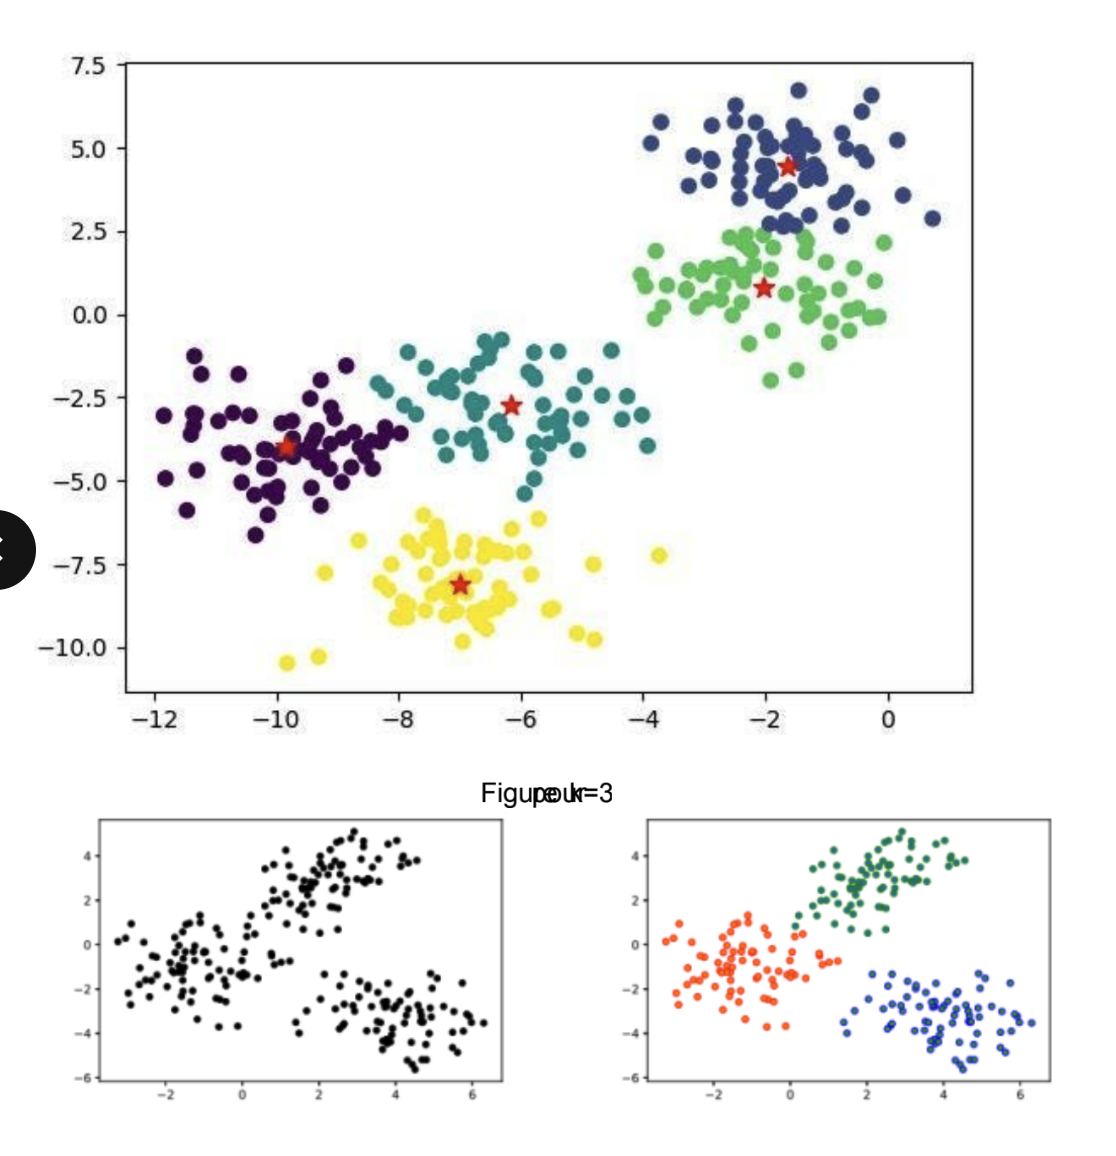
\includegraphics[width=0.3\linewidth]{exemple_kmean.png}
\captionof{figure}{\color{Green} Exemple classification avec sklearn}
\end{center}\vspace{1cm}

On peut mettre en place le pseudo-code suivant:

\begin{center}\vspace{1cm}
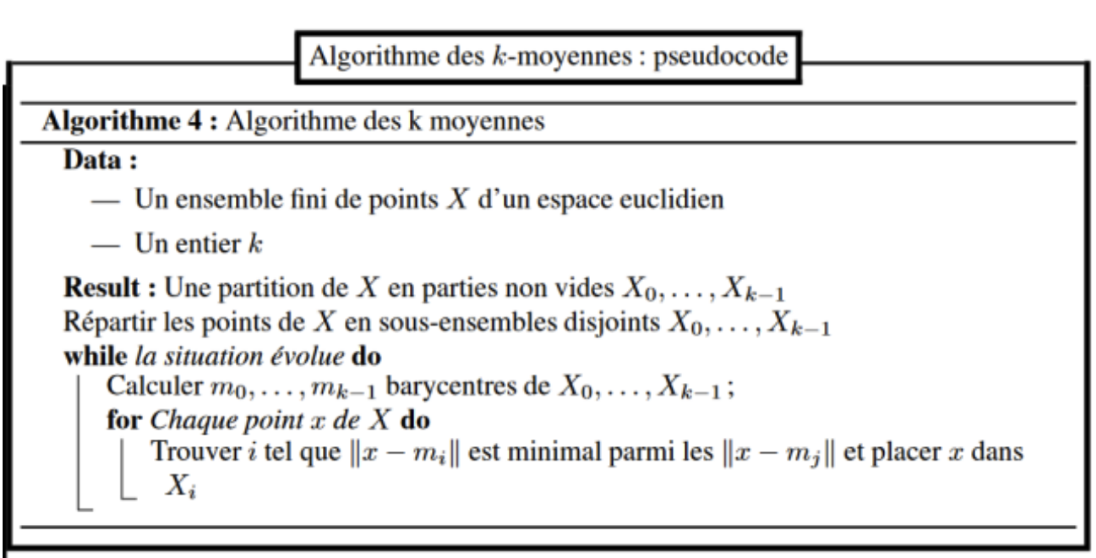
\includegraphics[width=0.3\linewidth]{pseudo_code.png}
\end{center}\vspace{1cm}
%----------------------------------------------------------------------------------------
%	CONCLUSIONS
%----------------------------------------------------------------------------------------

\color{DarkSlateGray} % Set the color back to DarkSlateGray for the rest of the content


\nocite{*} % Print all references regardless of whether they were cited in the poster or not
\bibliographystyle{plain} % Plain referencing style
\bibliography{sample} % Use the example bibliography file sample.bib

%----------------------------------------------------------------------------------------
%	ACKNOWLEDGEMENTS
%----------------------------------------------------------------------------------------

\section*{Pour aller plus loin}

\begin{enumerate}
    \item \href{https://scikit-learn.org}{Scikit-learn}.
    \item \href{https://fr.wikipedia.org/wiki/K-moyennes}{Wikipedia}
\end{enumerate}

%----------------------------------------------------------------------------------------

%\end{multicols}
\end{document}
